\chapter{利用例}
\label{chap:riyourei}

本章ではDrawWikiの利用例を紹介する。

\newpage

手書きメモ・イラストの内部に別の画像へのリンクが埋め込めるというDrawWikiの機能を活かした利用例を次に示す。

\section{アイデアスケッチ}
\label{drawiki:normalmemo}
スケッチをまとめる手段としてDrawWikiを活用することができる。
まずスケッチのテーマを示したメモを描き(図\ref{fig:ideasketch1})、そのテーマに沿ったスケッチ
(図\ref{fig:ideasketch2}、図\ref{fig:ideasketch3}、図\ref{fig:ideasketch4})にメモをリンクさせることで、
どのスケッチにアクセスしても共通のテーマを持つスケッチに到達することができる。
\begin{figure}[H] \begin{minipage}{0.5\hsize}
                      \begin{center} \fbox {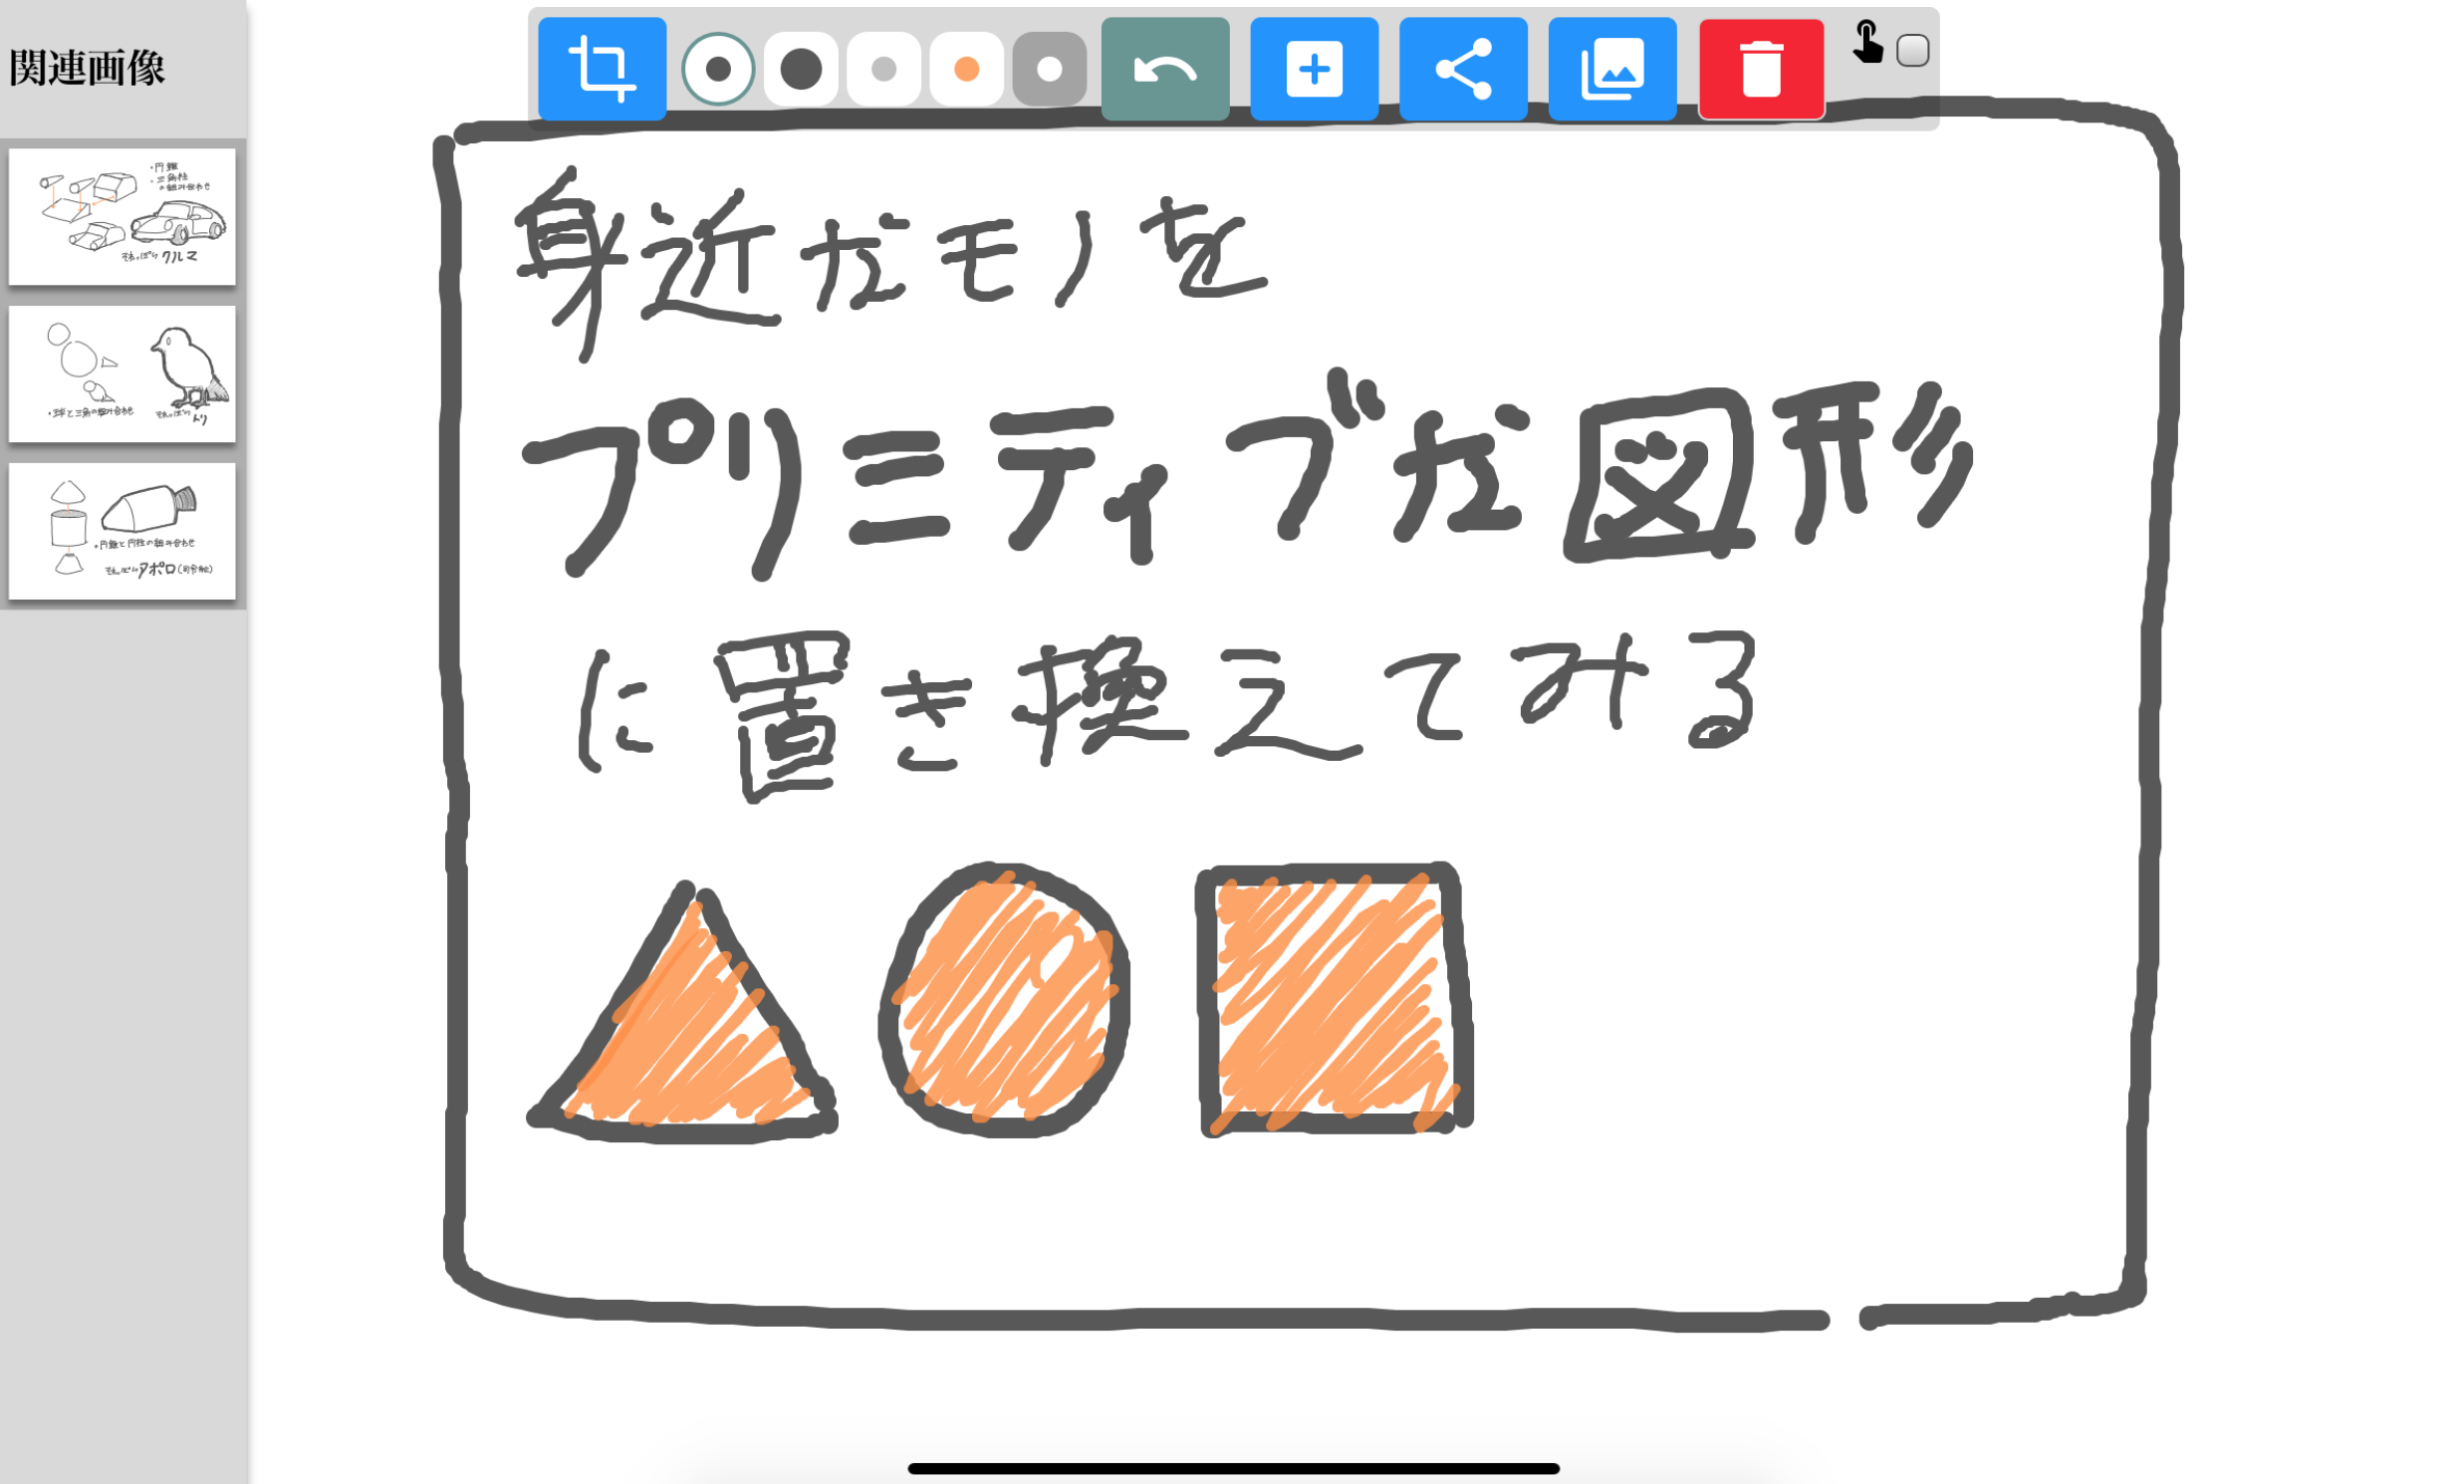
\includegraphics[width=70mm]{images/ideasketch1.png}}
                      \end{center} \caption{スケッチのテーマ} \label{fig:ideasketch1}
\end{minipage} \begin{minipage}{0.5\hsize}
                   \begin{center} \fbox {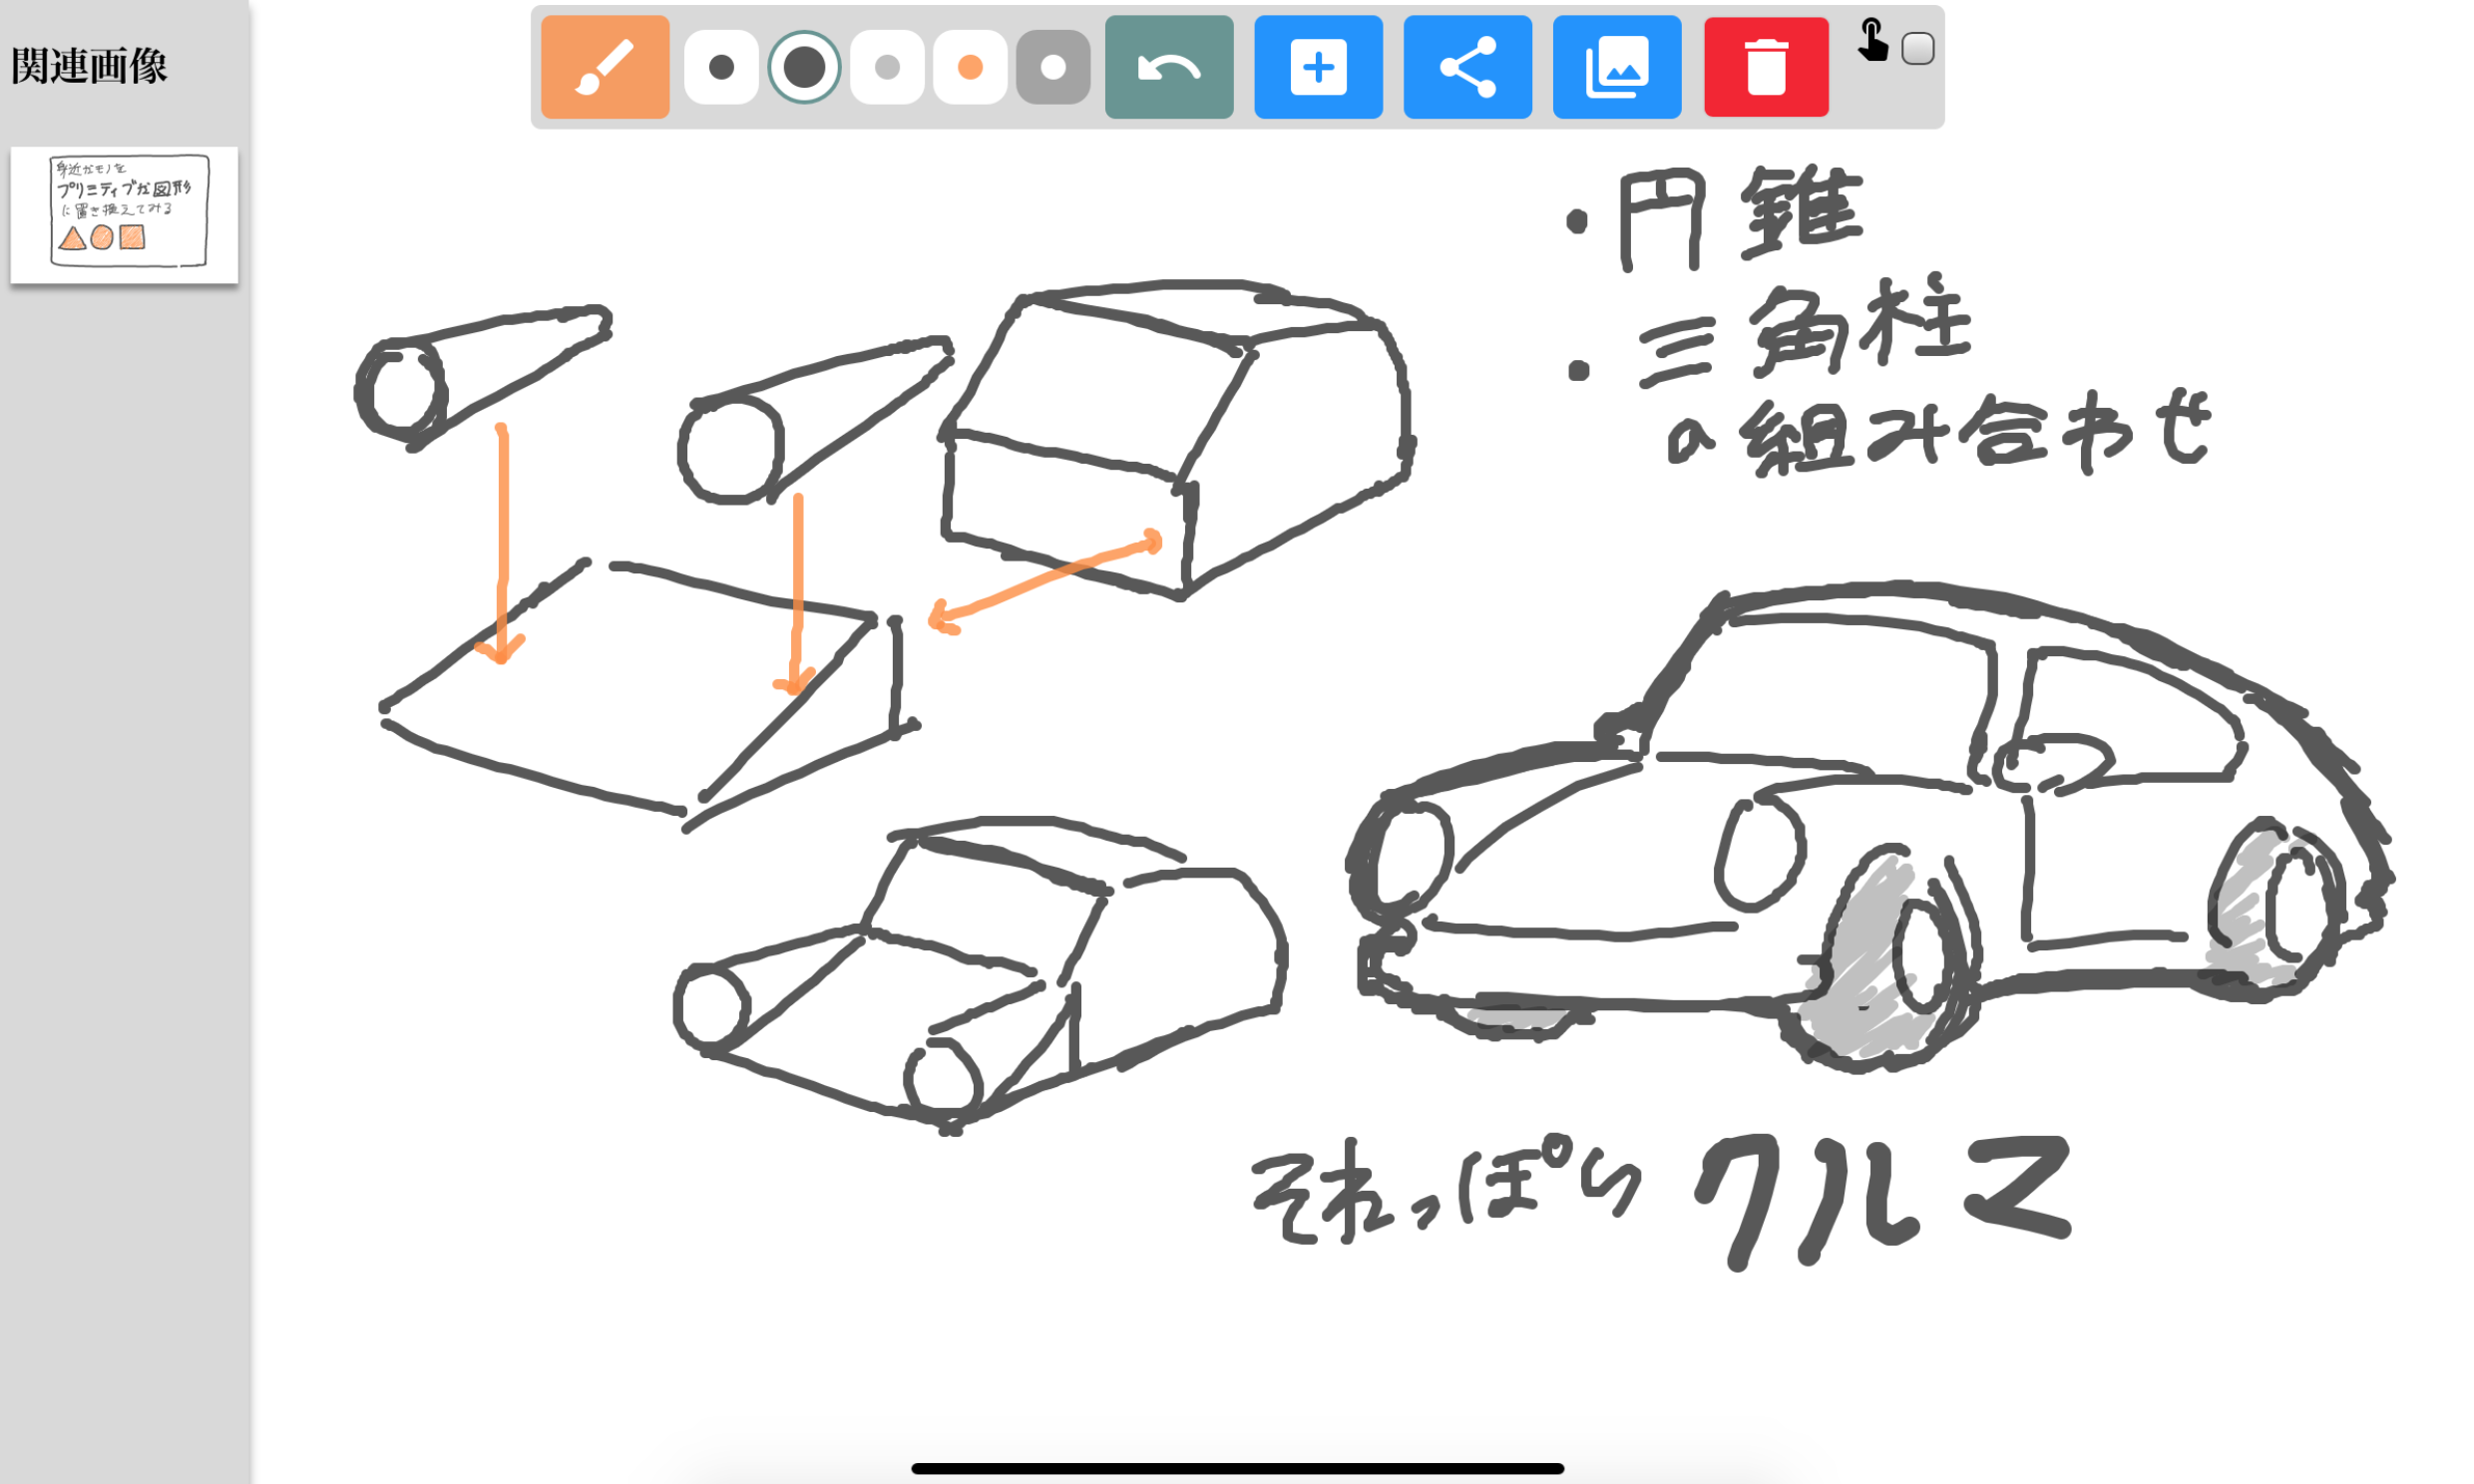
\includegraphics[width=70mm]{images/ideasketch2.png}}
                   \end{center} \caption{スケッチ例1} \label{fig:ideasketch2}
\end{minipage} \begin{minipage}{0.5\hsize}
                      \begin{center} \fbox {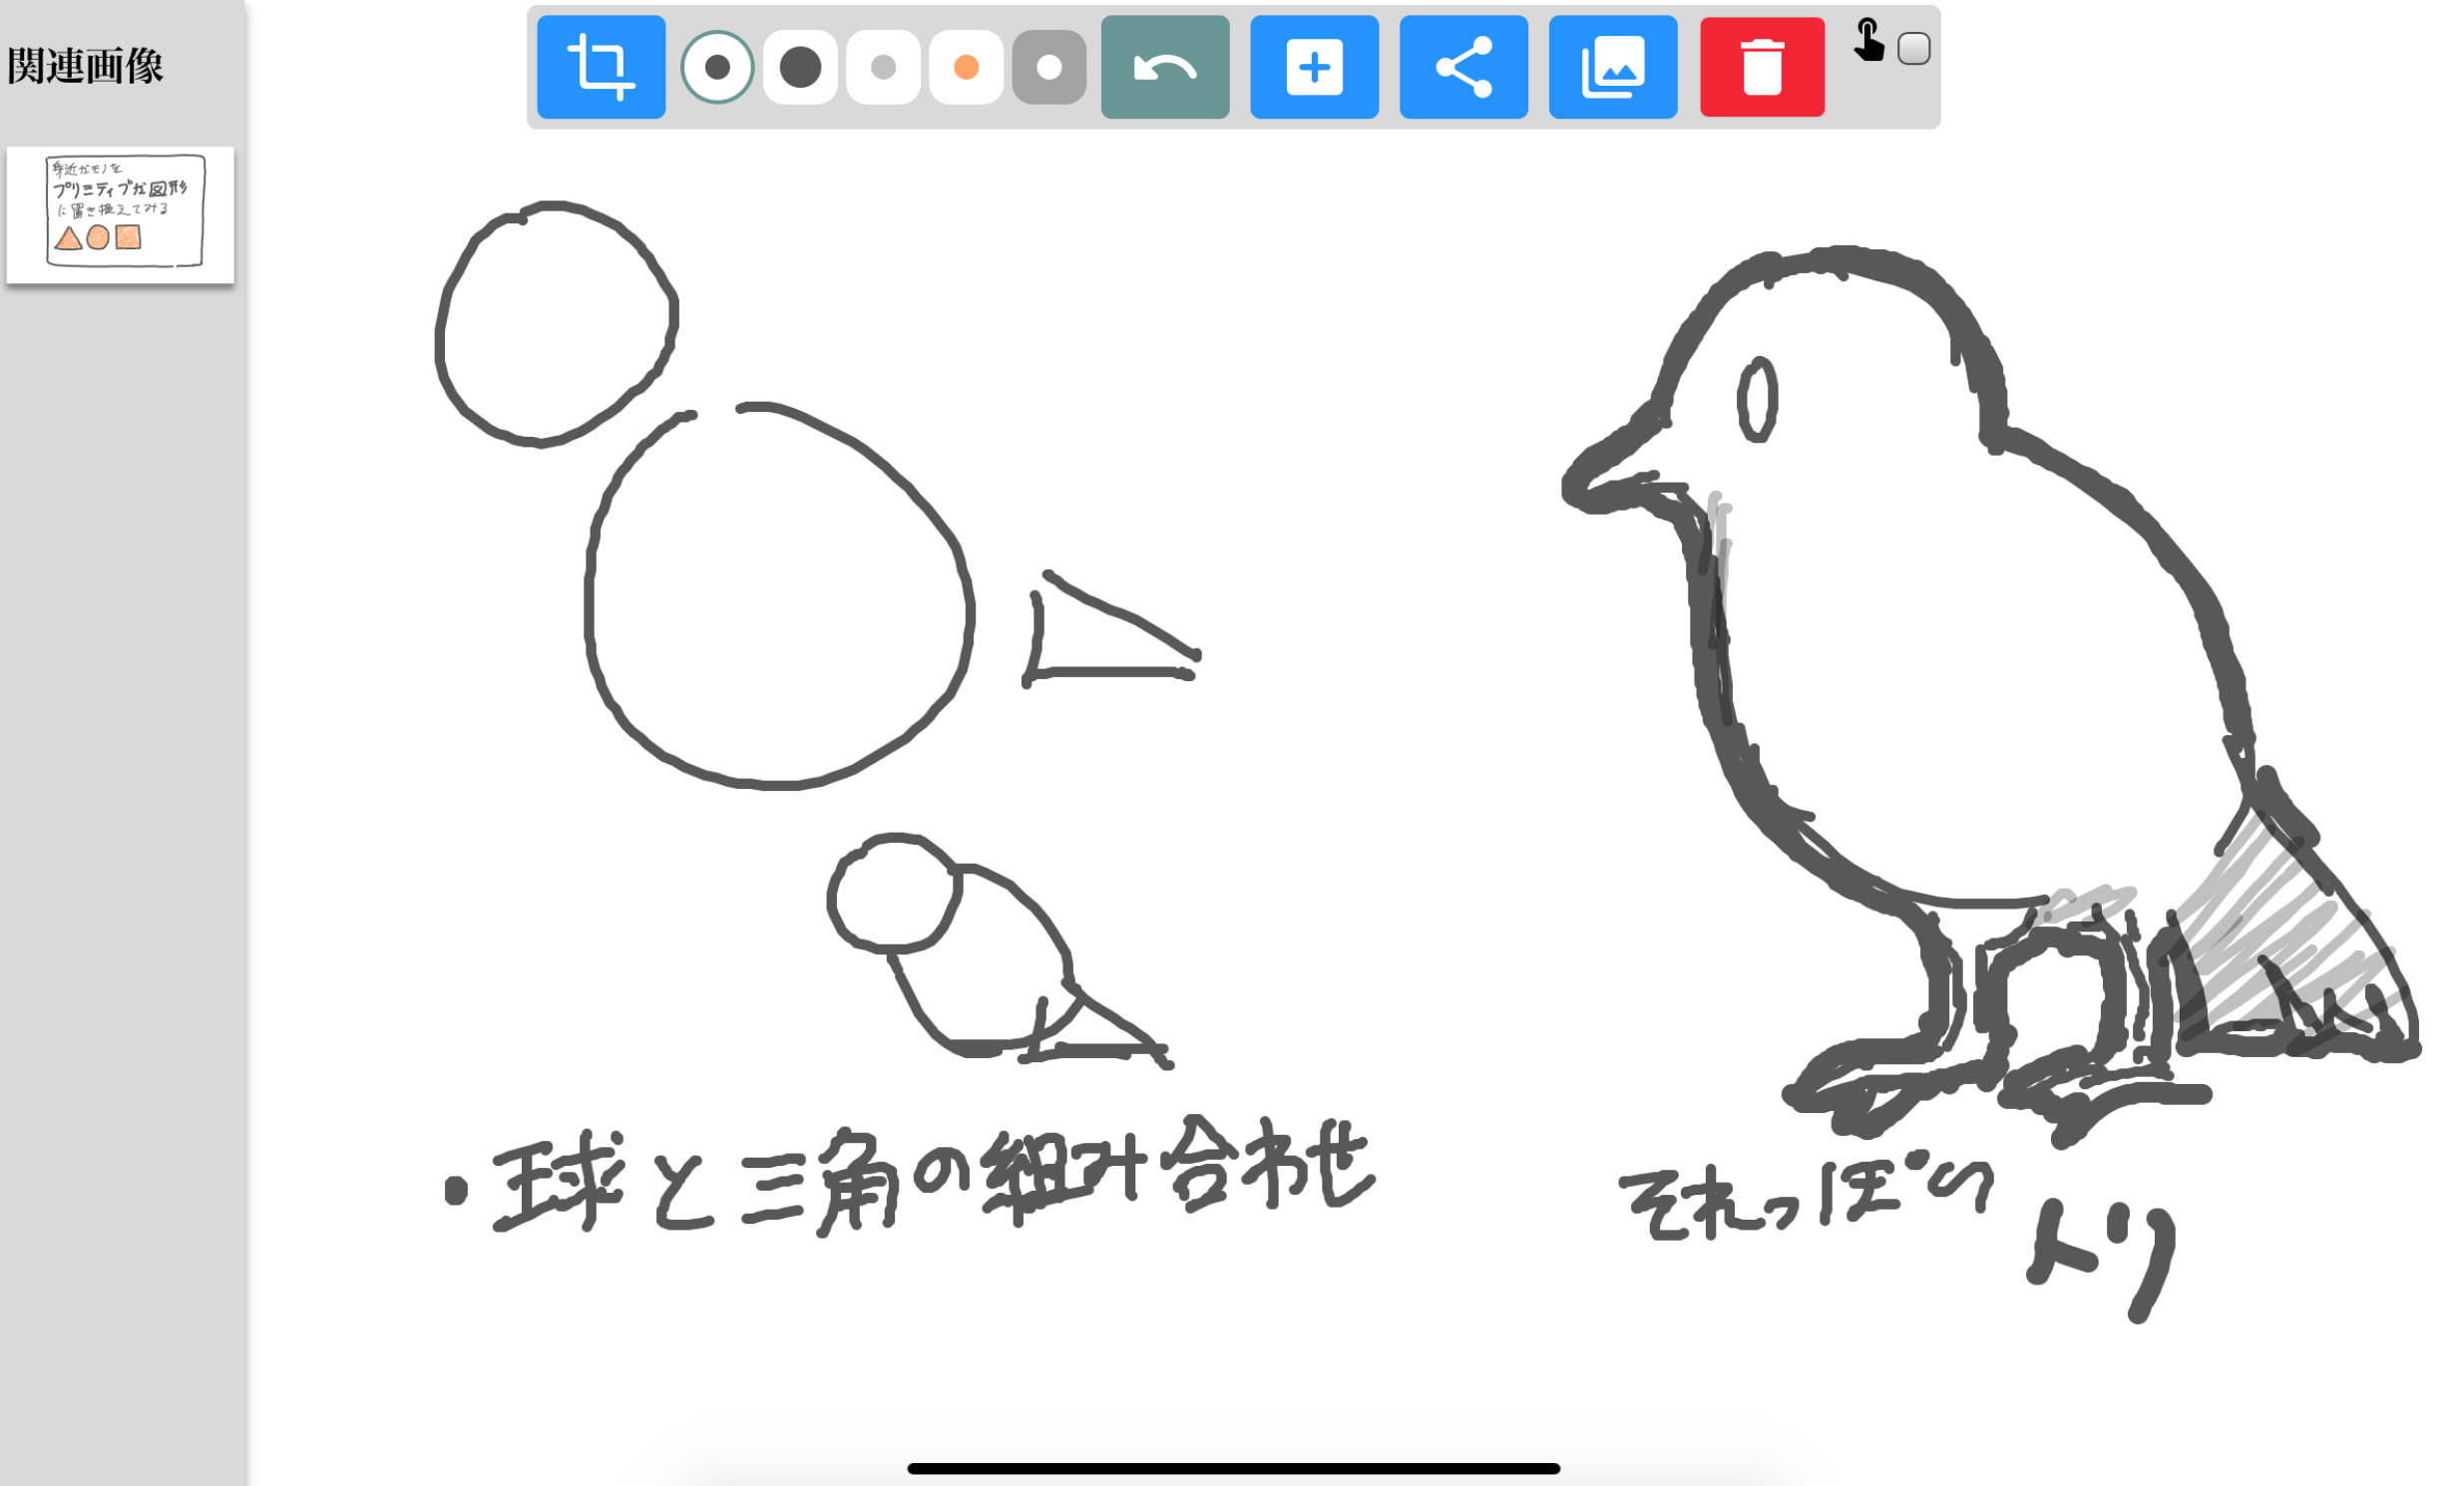
\includegraphics[width=70mm]{images/ideasketch3.png}}
                      \end{center} \caption{スケッチ例2} \label{fig:ideasketch3}
\end{minipage} \begin{minipage}{0.5\hsize}
                   \begin{center} \fbox {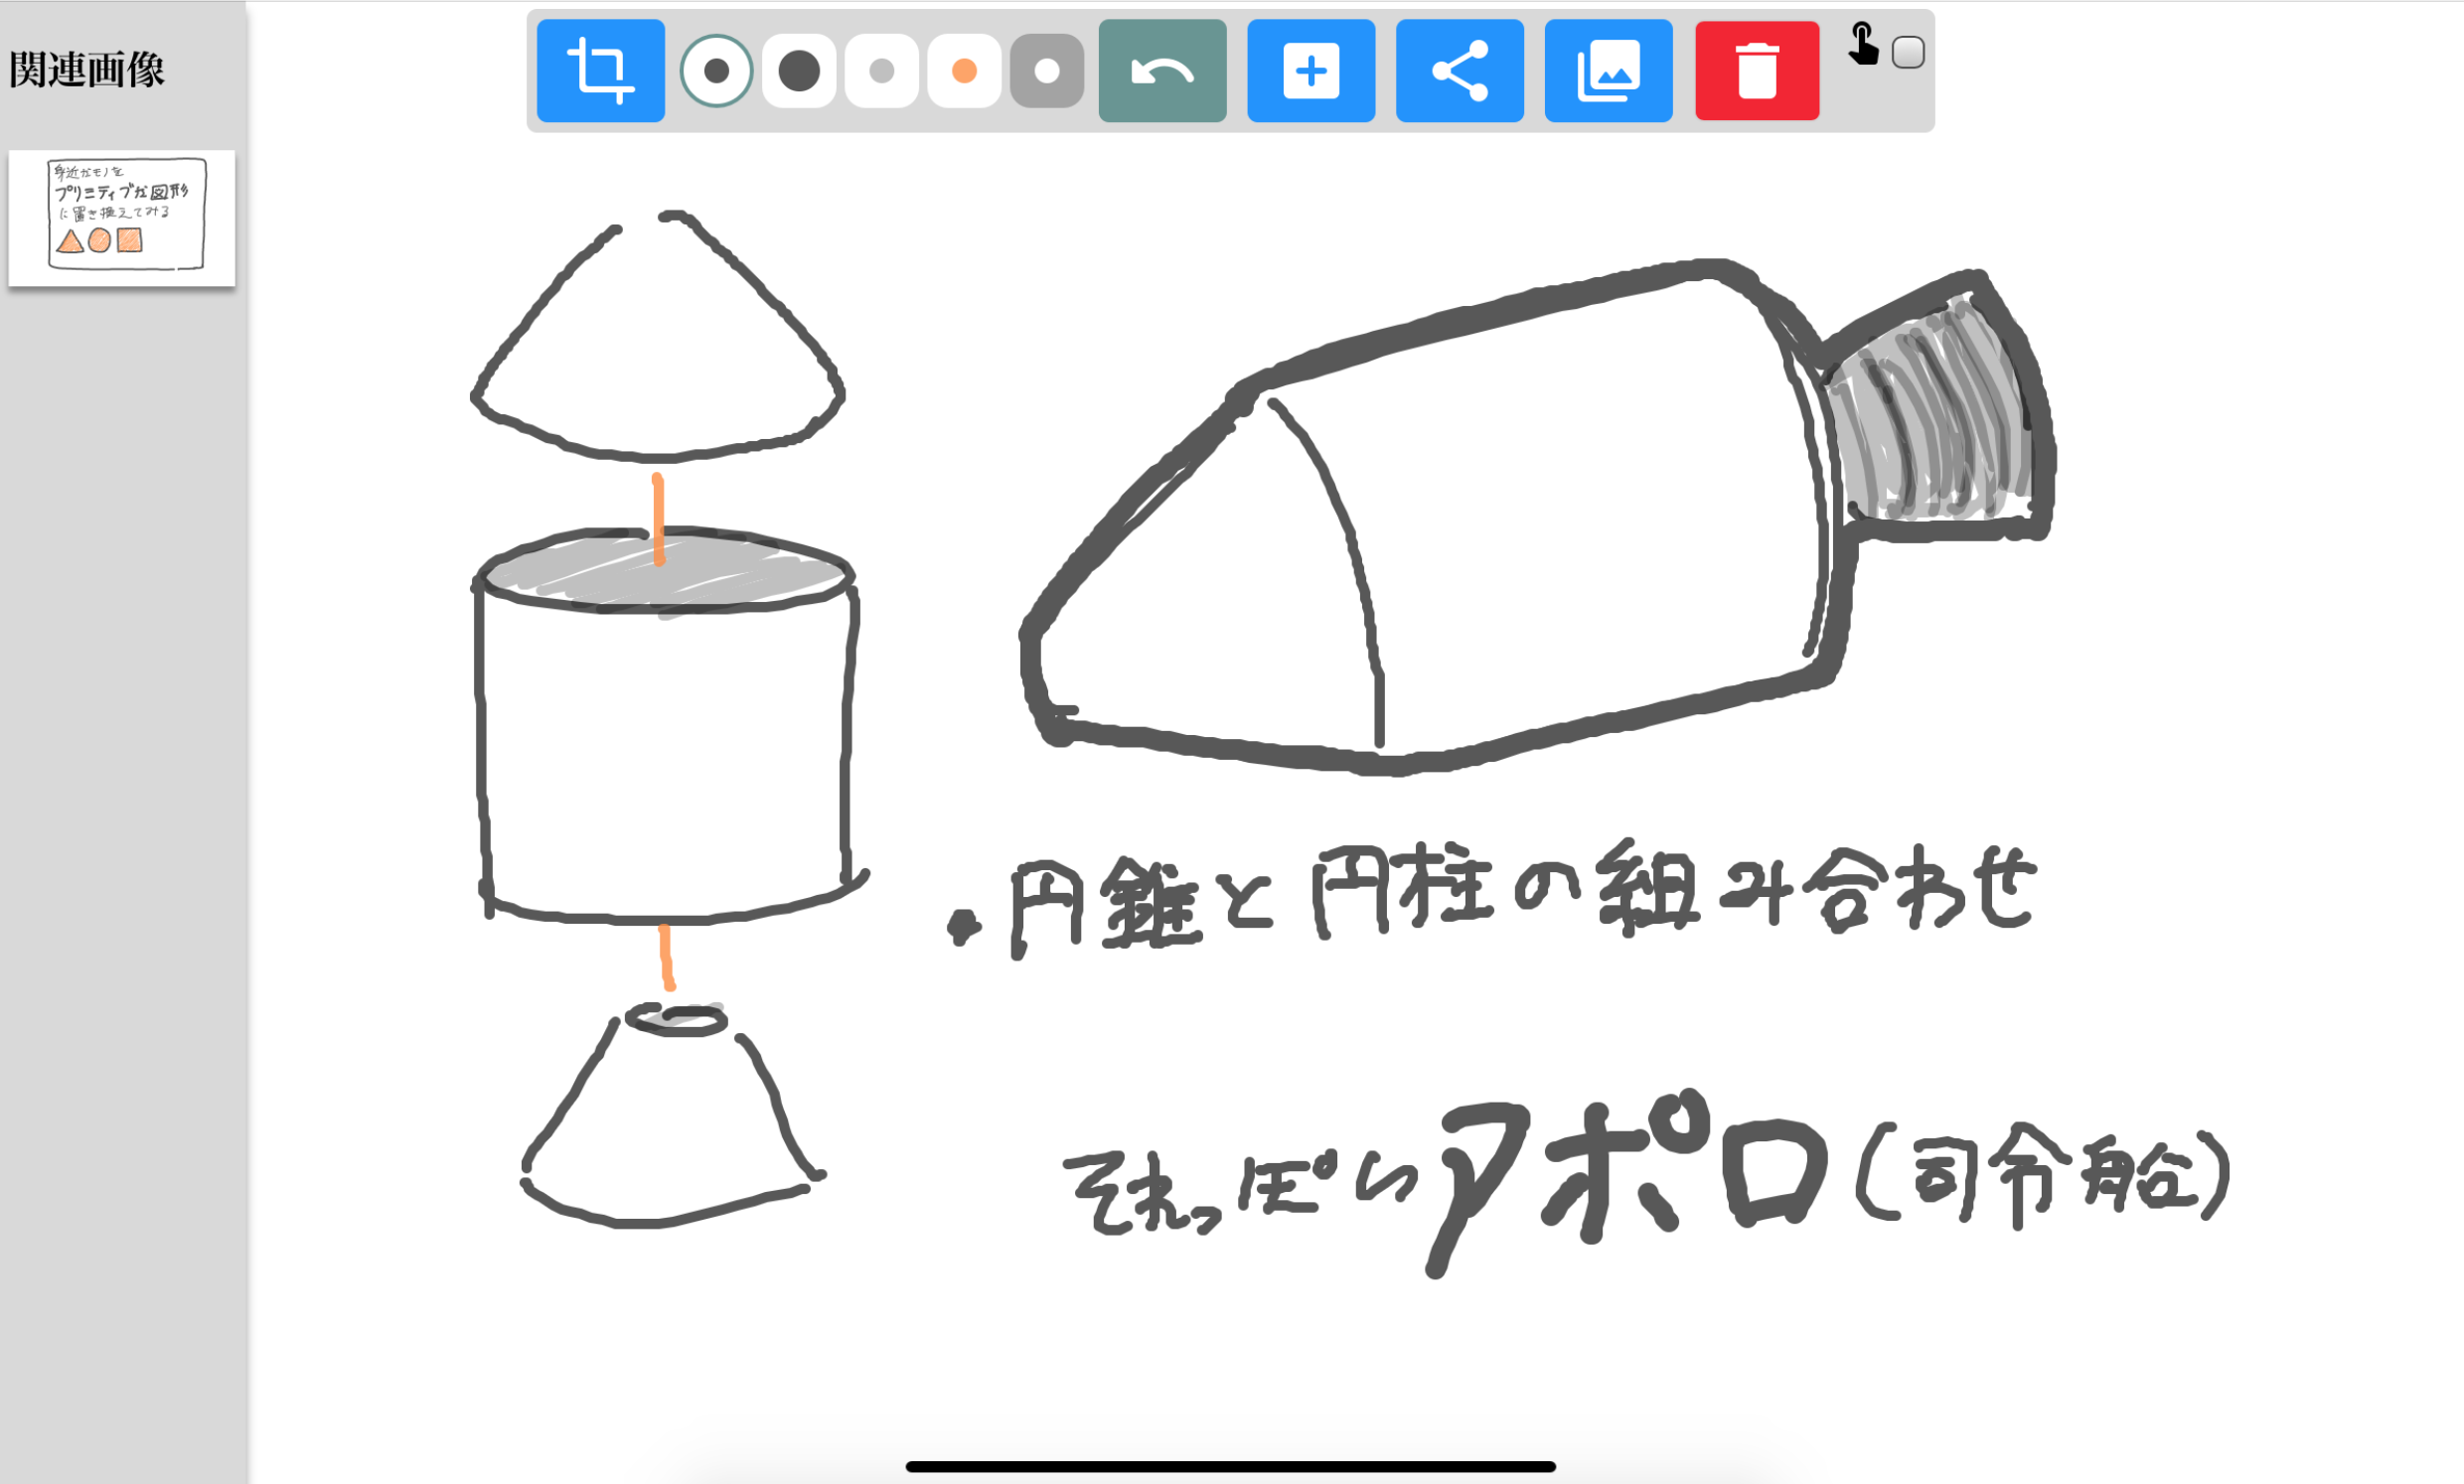
\includegraphics[width=70mm]{images/ideasketch4.png}}
                   \end{center} \caption{スケッチ例3} \label{fig:ideasketch4}
\end{minipage}
\end{figure}


\section{場所の説明}
\label{drawiki:map}
地理情報なども手書きメモが得意とする領域である。図\ref{fig:drawwikimap1}はDrawWikiによって描かれた
手書きの非公式キャンパスマップである。青色で強調表示されている部分がキャンパスにおけるバイク駐輪場であり、
その領域にはバイク駐輪場の概観を描いたイラスト(図\ref{fig:drawwikimap2})へのリンクが埋め込まれている。通常の地図には記されていない
特殊な場所に関する情報を表現・共有したい場合にもこの機能は有効である。

\begin{figure}[H] \begin{minipage}{0.5\hsize}
                      \begin{center} \fbox {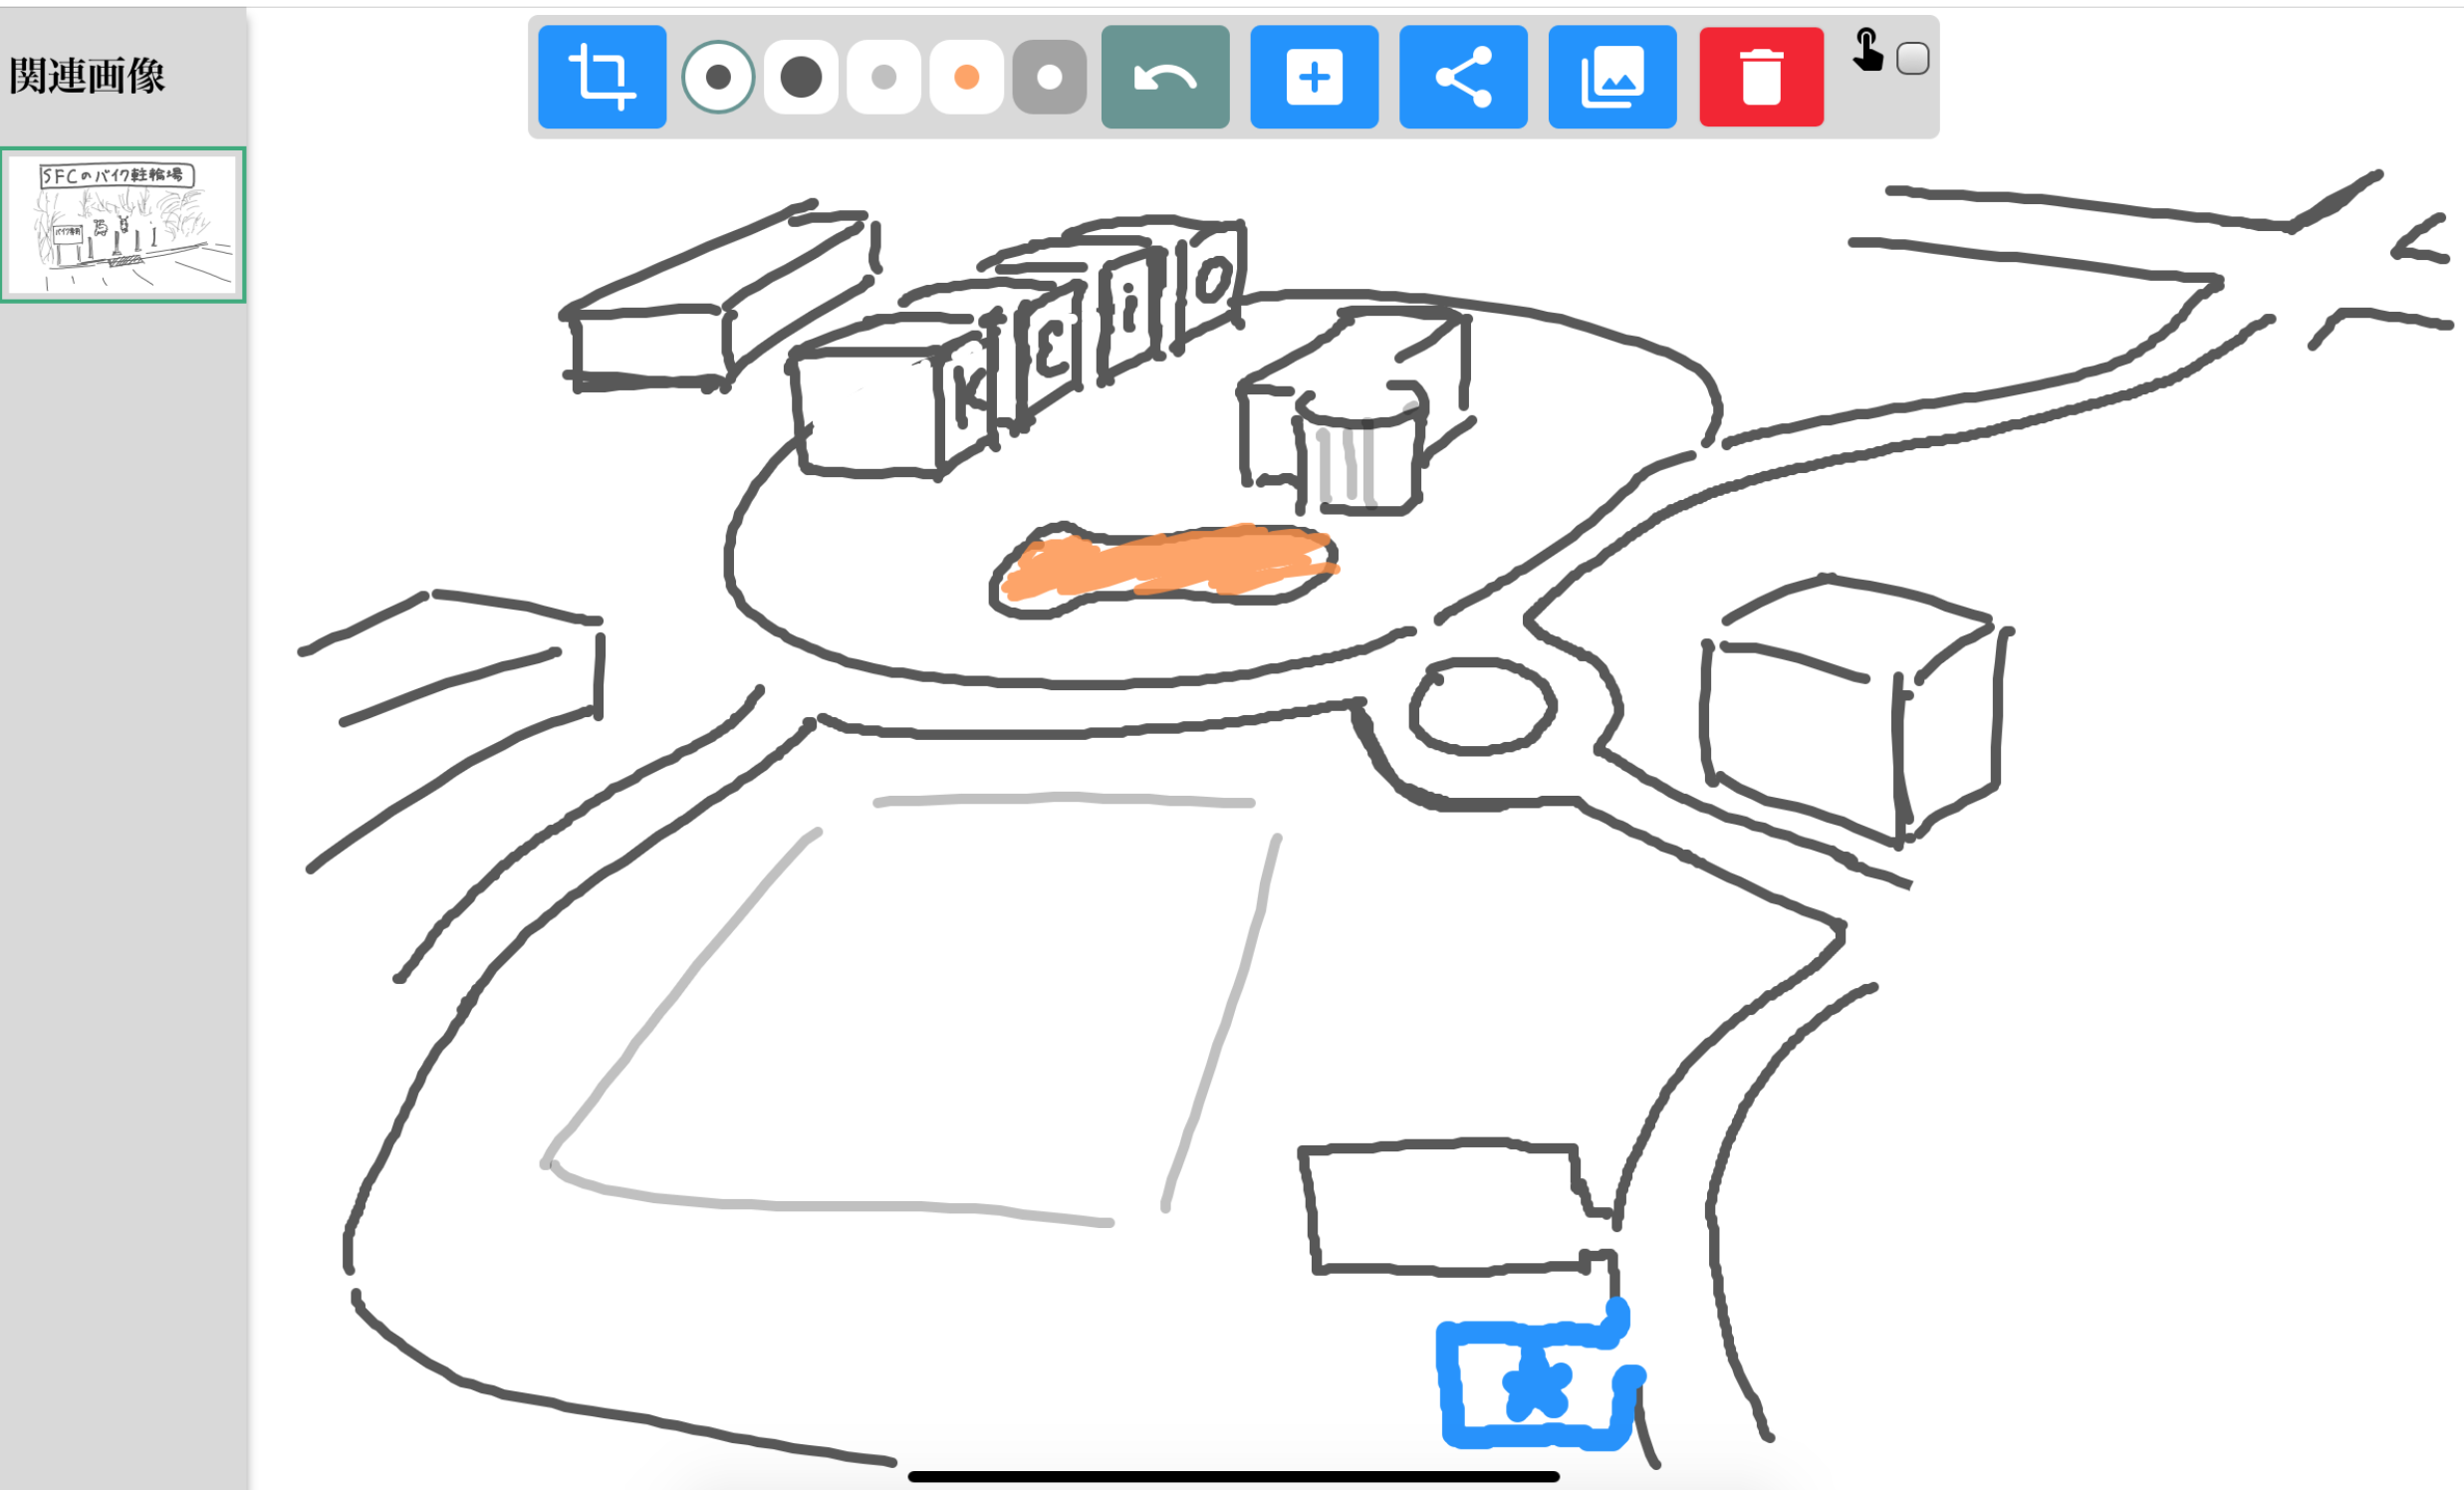
\includegraphics[width=70mm]{images/drawikimap1.png}}
                      \end{center} \caption{非公式キャンバスマップ} \label{fig:drawwikimap1}
\end{minipage} \begin{minipage}{0.5\hsize}
                   \begin{center} \fbox {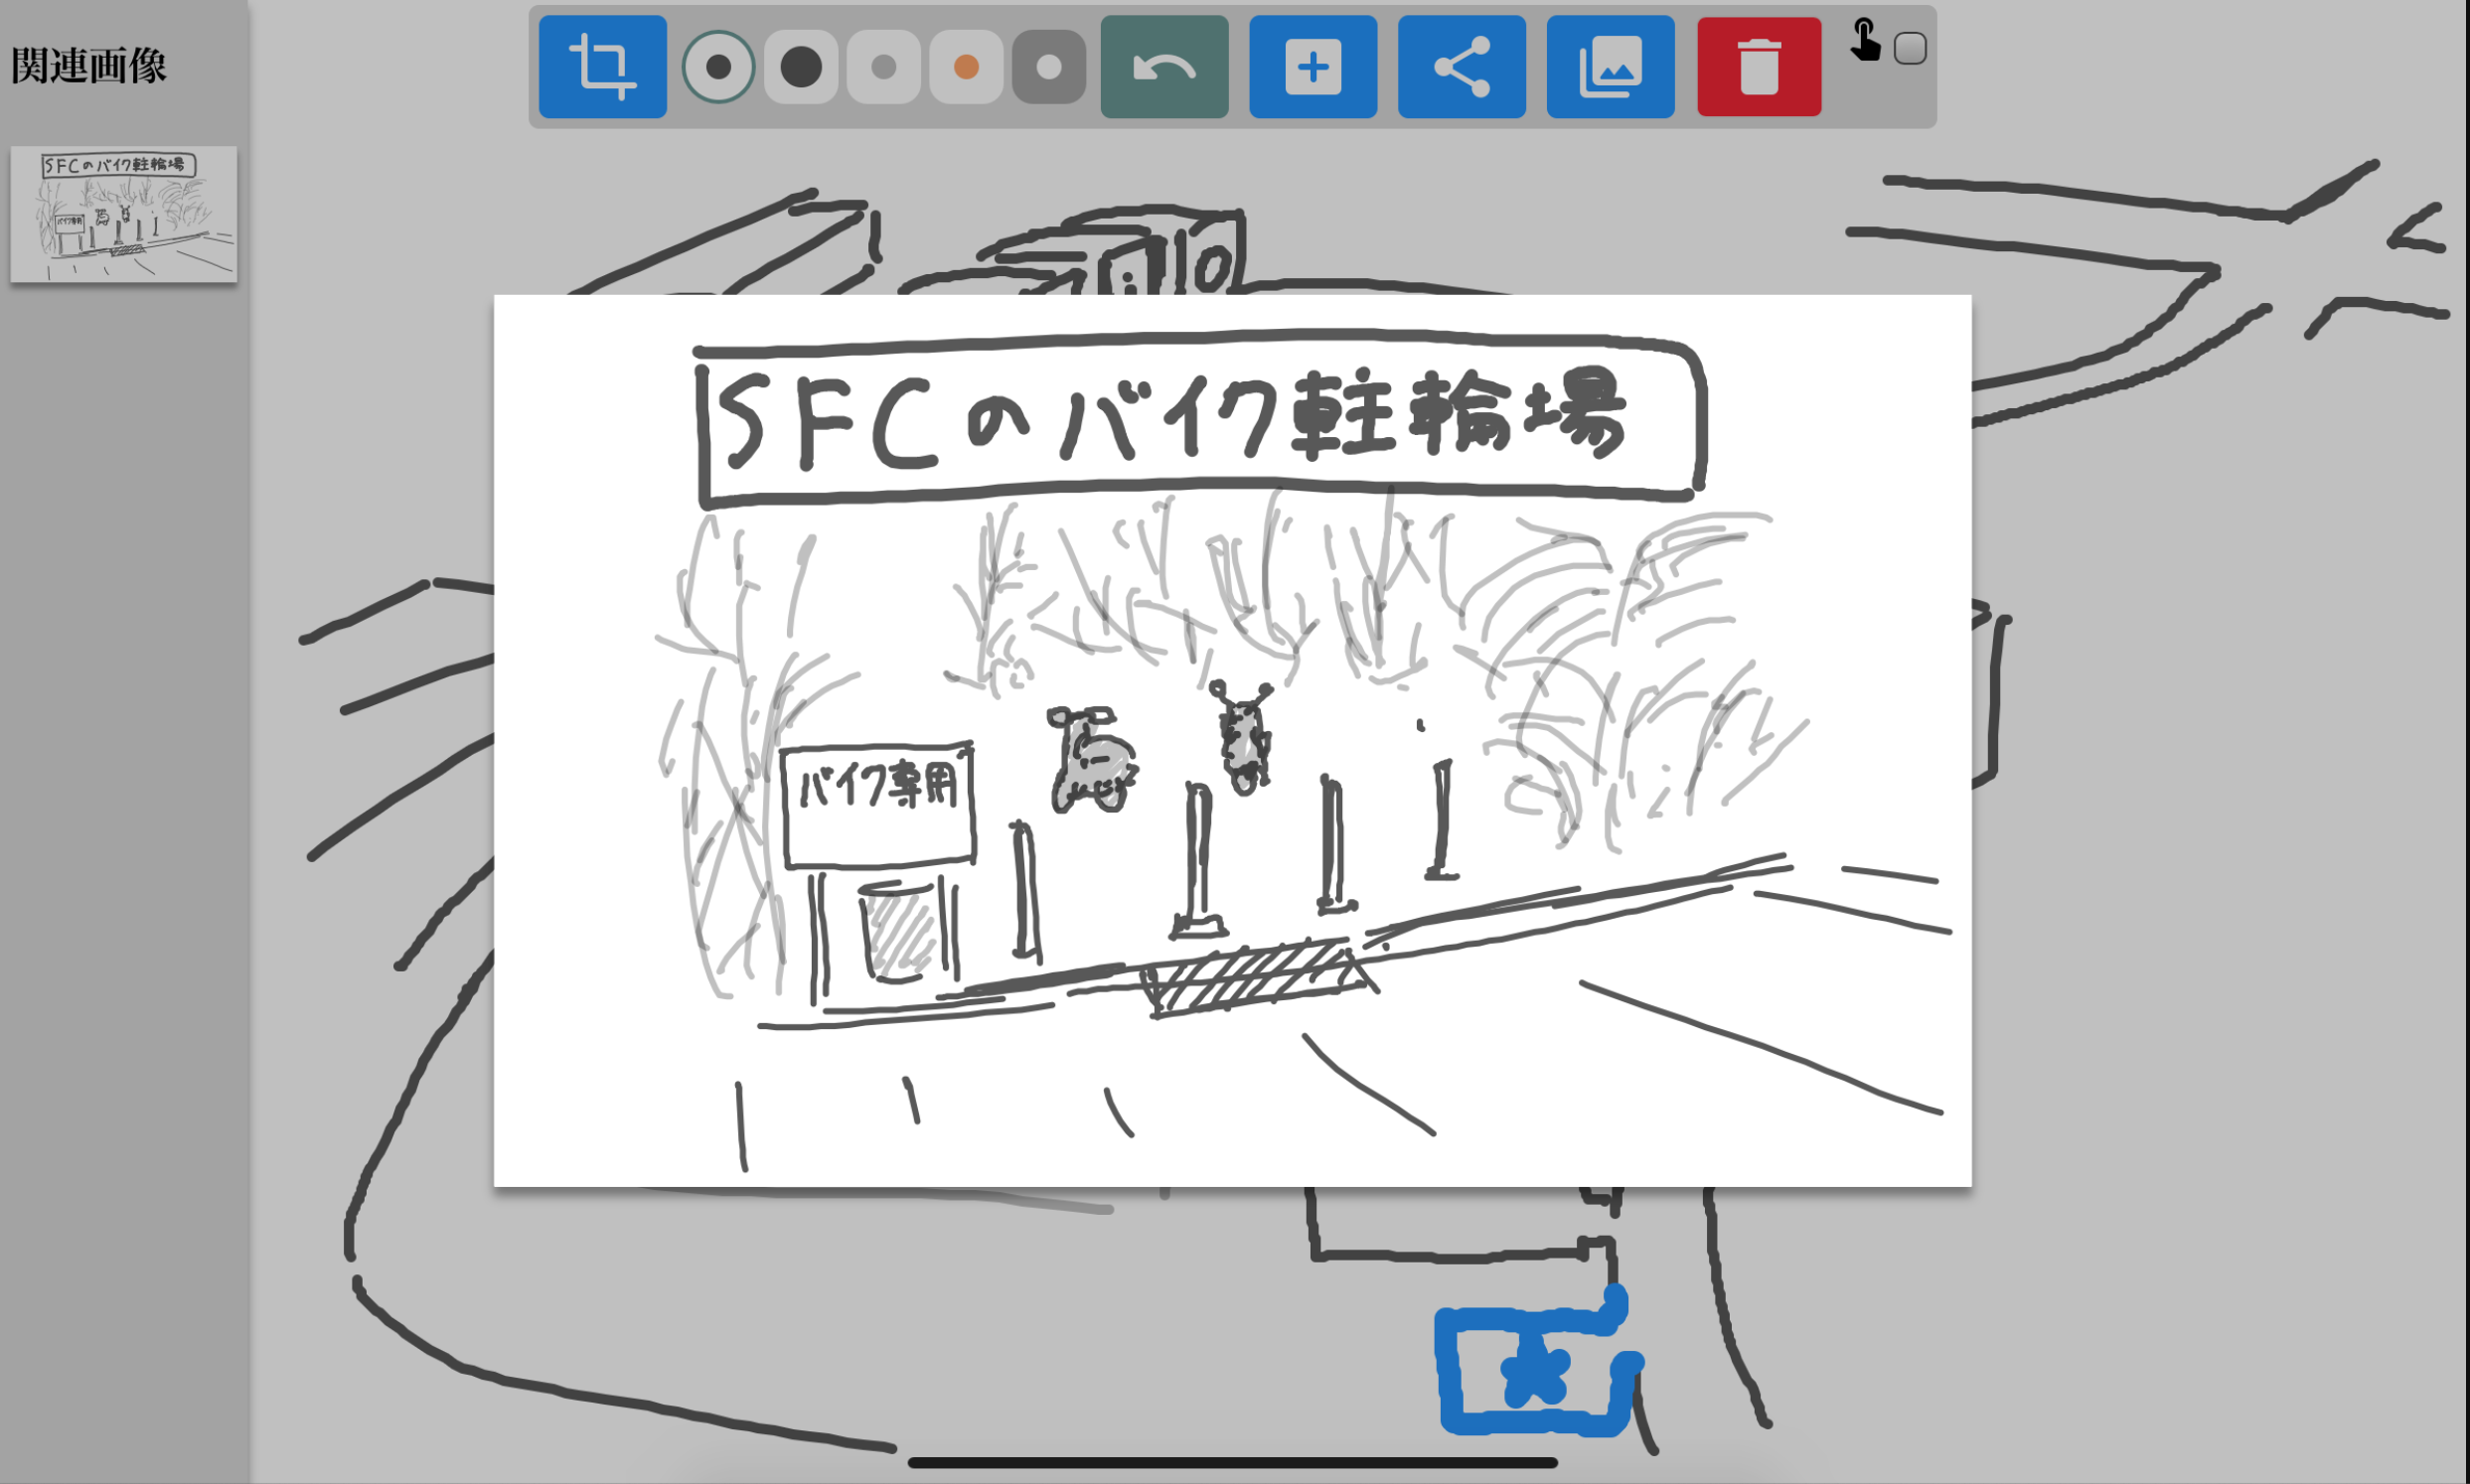
\includegraphics[width=70mm]{images/drawwikimap2.png}}
                   \end{center} \caption{バイク駐輪場の場所と概観} \label{fig:drawwikimap2}
\end{minipage}
\end{figure}



\section{スケッチによるソフトウェアのモックアップの作成}
\label{drawiki:mockup}
ソフトウェアの画面や挙動を設計する際に、柔軟な表現が可能な手書きスケッチを用いることは有効なデザインプラクティスとして知られている。
DrawWikiを開発する際も、機能や画面全体のデザインを考える際にDrawWikiを用いてスケッチを行いながら検討した。
リンクが埋め込まれた要素をクリックするとリンク先の画像が表示される(図\ref{fig:protodrawwiki2})ことから、これをインタラクションや画面遷移に見立てることにより
図\ref{fig:protodrawwiki1}のようなナビゲーションを伴ったソフトウェアのモックアップを手書きスケッチによって作成することができる。

\begin{figure}[H] \begin{minipage}{0.5\hsize}
                      \begin{center} \fbox {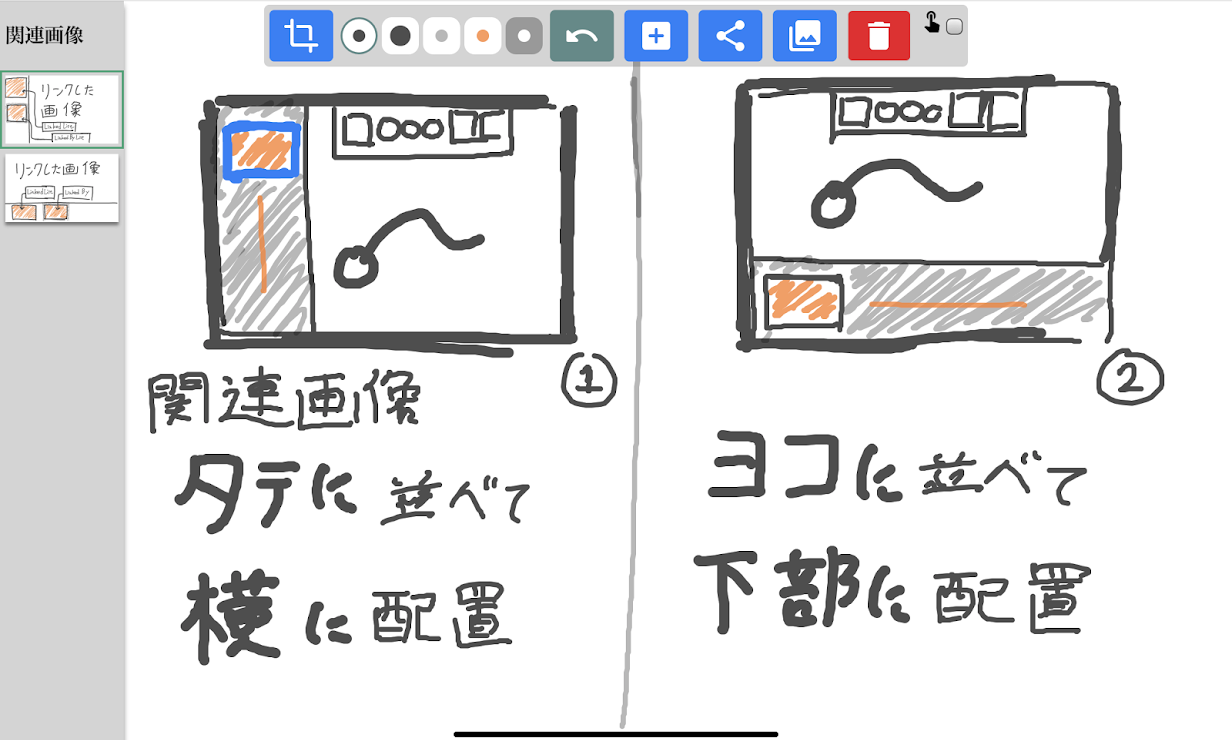
\includegraphics[width=70mm]{images/mockup1.png}}
                      \end{center} \caption{DrawWikを用いて作成されたDrawwikiのモックアップ} \label{fig:protodrawwiki1}
\end{minipage} \begin{minipage}{0.5\hsize}
                   \begin{center} \fbox {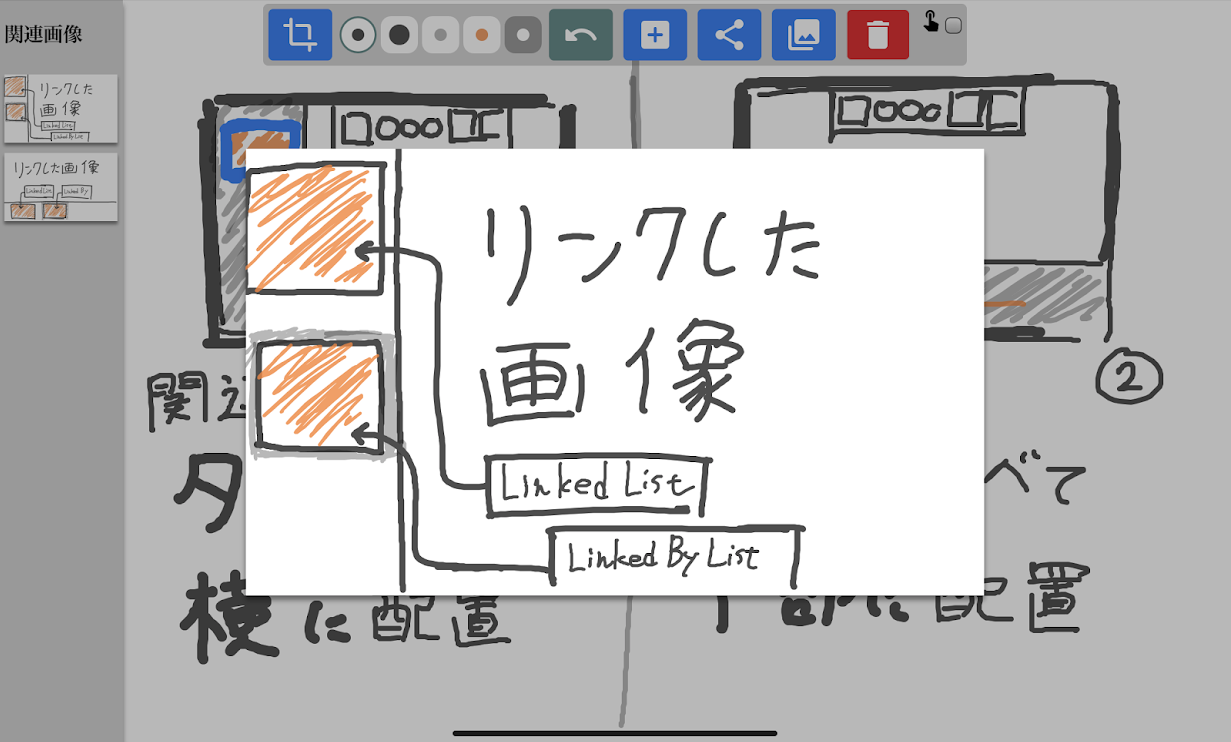
\includegraphics[width=70mm]{images/mockup2.png}}
                   \end{center} \caption{インタラクションとして再現されるダイアログ} \label{fig:protodrawwiki2}
\end{minipage}
\end{figure}


\section{インタラクティブな図解}
\label{drawiki:zukai}
自動車等の整備を行う際は、製品マニュアルを熟読することで構造を理解し、交換すべき部品をパーツリストで確認し、さらに
取り付けに必要なワッシャ・ボルトのサイズやそれらの適正な締め付けトルクを念頭に置いた上で行う必要があるが、それらの情報は
異なるページや冊子に分かれて記載されていることが一般的であり、参照が大変である。(図\ref{fig:partslist}, 図\ref{fig:manual})

\begin{figure}[H] \begin{minipage}{0.5\hsize}
                      \begin{center} \fbox {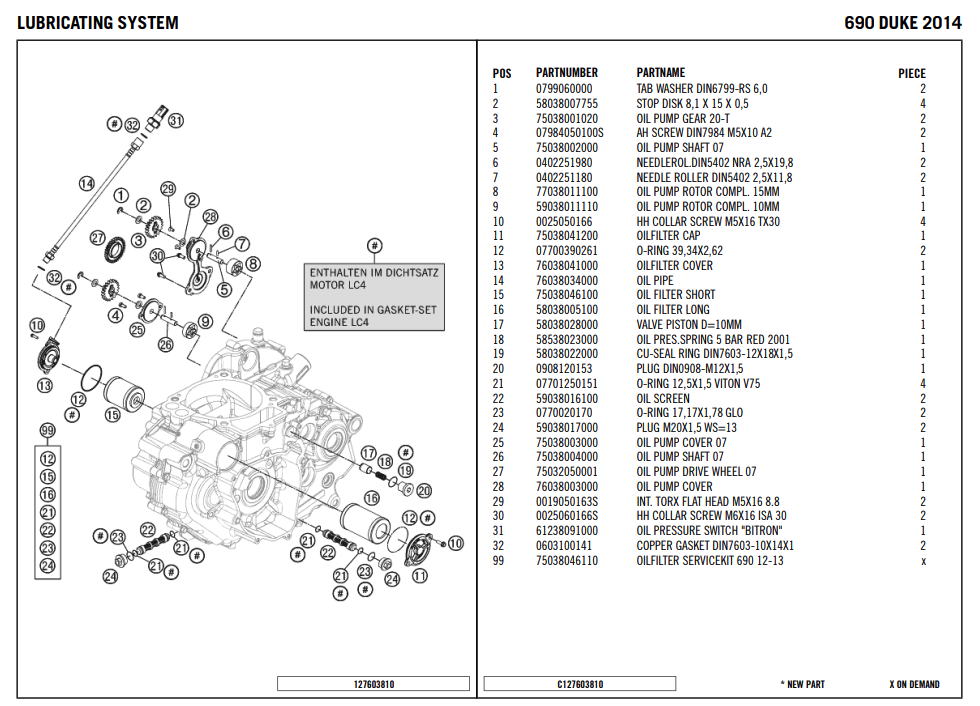
\includegraphics[width=70mm]{images/partslist.png}}
                      \end{center} \caption{既存のパーツリスト} \label{fig:partslist}
\end{minipage} \begin{minipage}{0.5\hsize}
                   \begin{center} \fbox {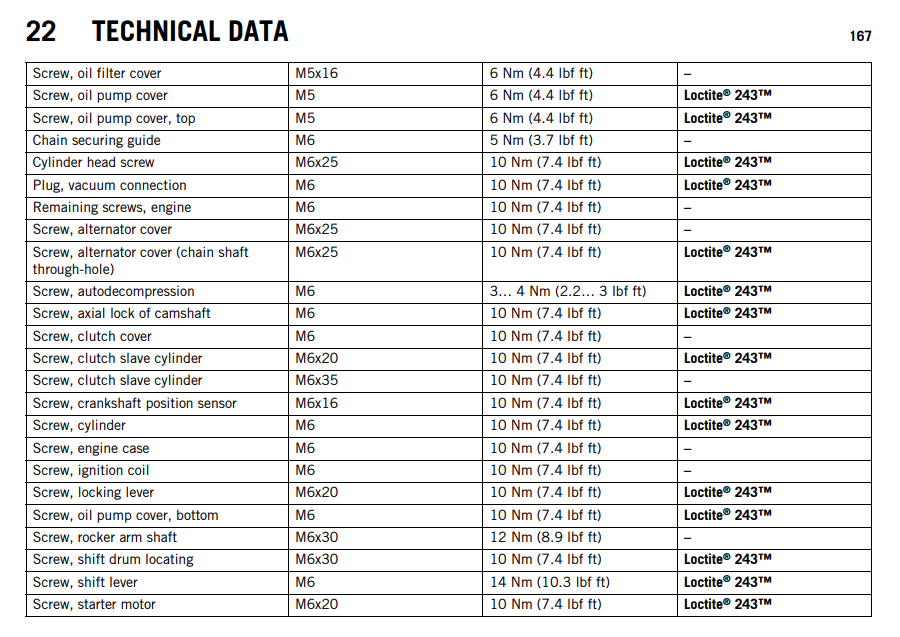
\includegraphics[width=70mm]{images/manual1.png}}
                   \end{center} \caption{既存の部品情報リスト} \label{fig:manual}
\end{minipage}
\end{figure}

\begin{figure}[H] \begin{minipage}{0.5\hsize}
                      \begin{center} \fbox {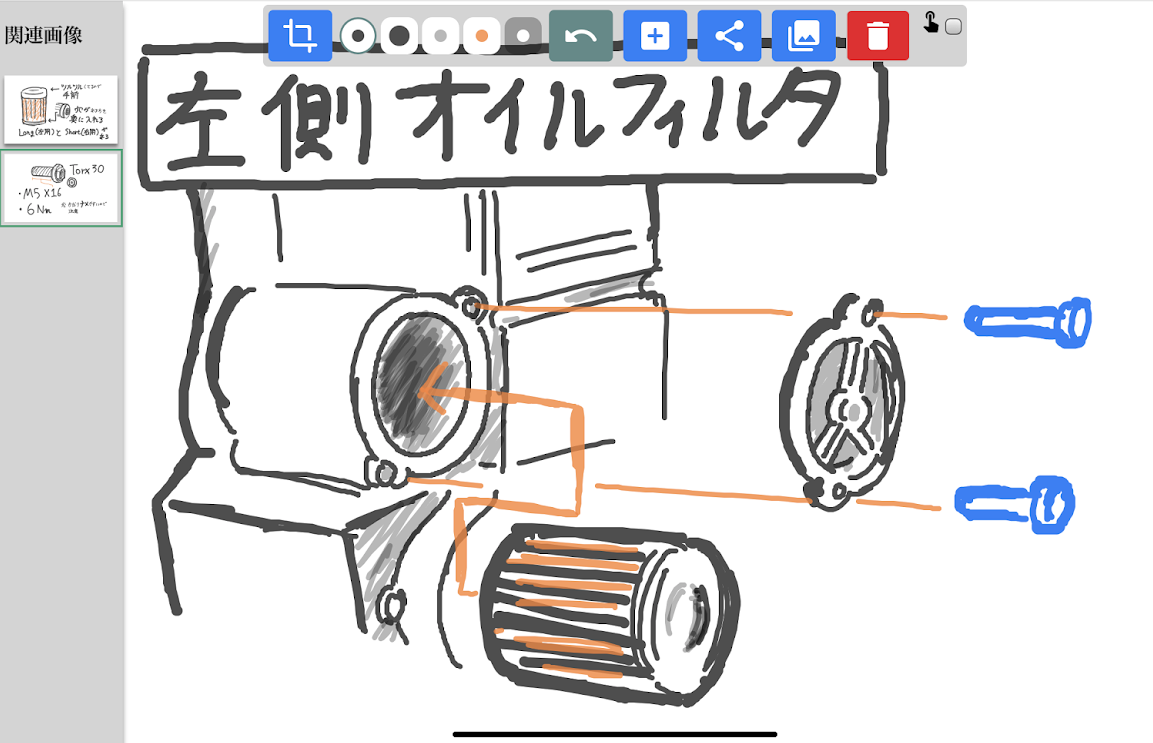
\includegraphics[width=70mm]{images/mymanual1.png}}
                      \end{center} \caption{DrawWikiによる自作整備メモ} \label{fig:oremanual1}
\end{minipage} \begin{minipage}{0.5\hsize}
                   \begin{center} \fbox {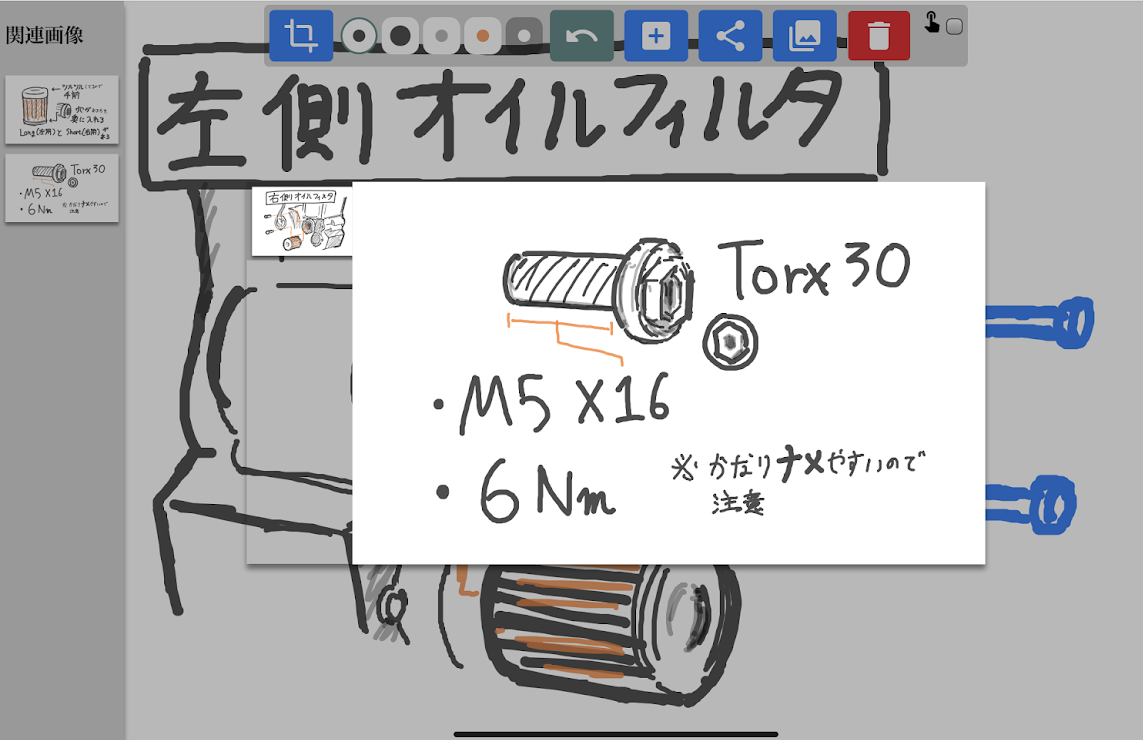
\includegraphics[width=70mm]{images/mymanual2.png}}
                   \end{center} \caption{関連情報を表示した画面} \label{fig:oremanual2}
\end{minipage}
\end{figure}

DrawWikiでは製品の構造を理解しやすいよう自由なレイアウトで簡潔に描いたメモ(図\ref{fig:oremanual1})に、部品や組み立てに要する注意等のリストが描かれた
別のメモ(図\ref{fig:oremanual2})をリンクさせることで、
必要な情報へ素早くアクセスする手段を確保しながら、画面が注釈で埋まることのない視認性に優れた図解を作成することが可能である。
またリンク構造によって同じ部品や工具を用いる他のメモも推薦されるため、整備の手順を考える手助けとなる効果もある。

\section{ナレッジの共有と共同編集}
DrawWikiによって作成された全てのメモやイラストにはURLが割り振られており、誰でもアクセスし編集することができる。
公開されている手書きメモに対する別のユーザーからの内容の追記やリンクの追加等の操作にも対応しているため
手書きメモ・イラストに対してWikiのようなコラボレーションを行うことを可能にしている。

\section{まとめ}
本章では、本システムによって実現可能な、手書きメモ・イラストが持つ柔軟な表現力と
リンクによる関連情報の表示等の機能を活かした利用例について述べた。
手書きメモやハイパーリンク、Wikiの持つ潜在的な表現力や拡張性から、本章で述べた利用例に限らず様々な応用が可能であると考えられる。